\chapter{Results}
\label{chapter:results}


The relationship between resistance and pressure is non-linear (as expected for Velostat).\begin{figure}[b]
    \vspace{-0.7cm}
      \centering
      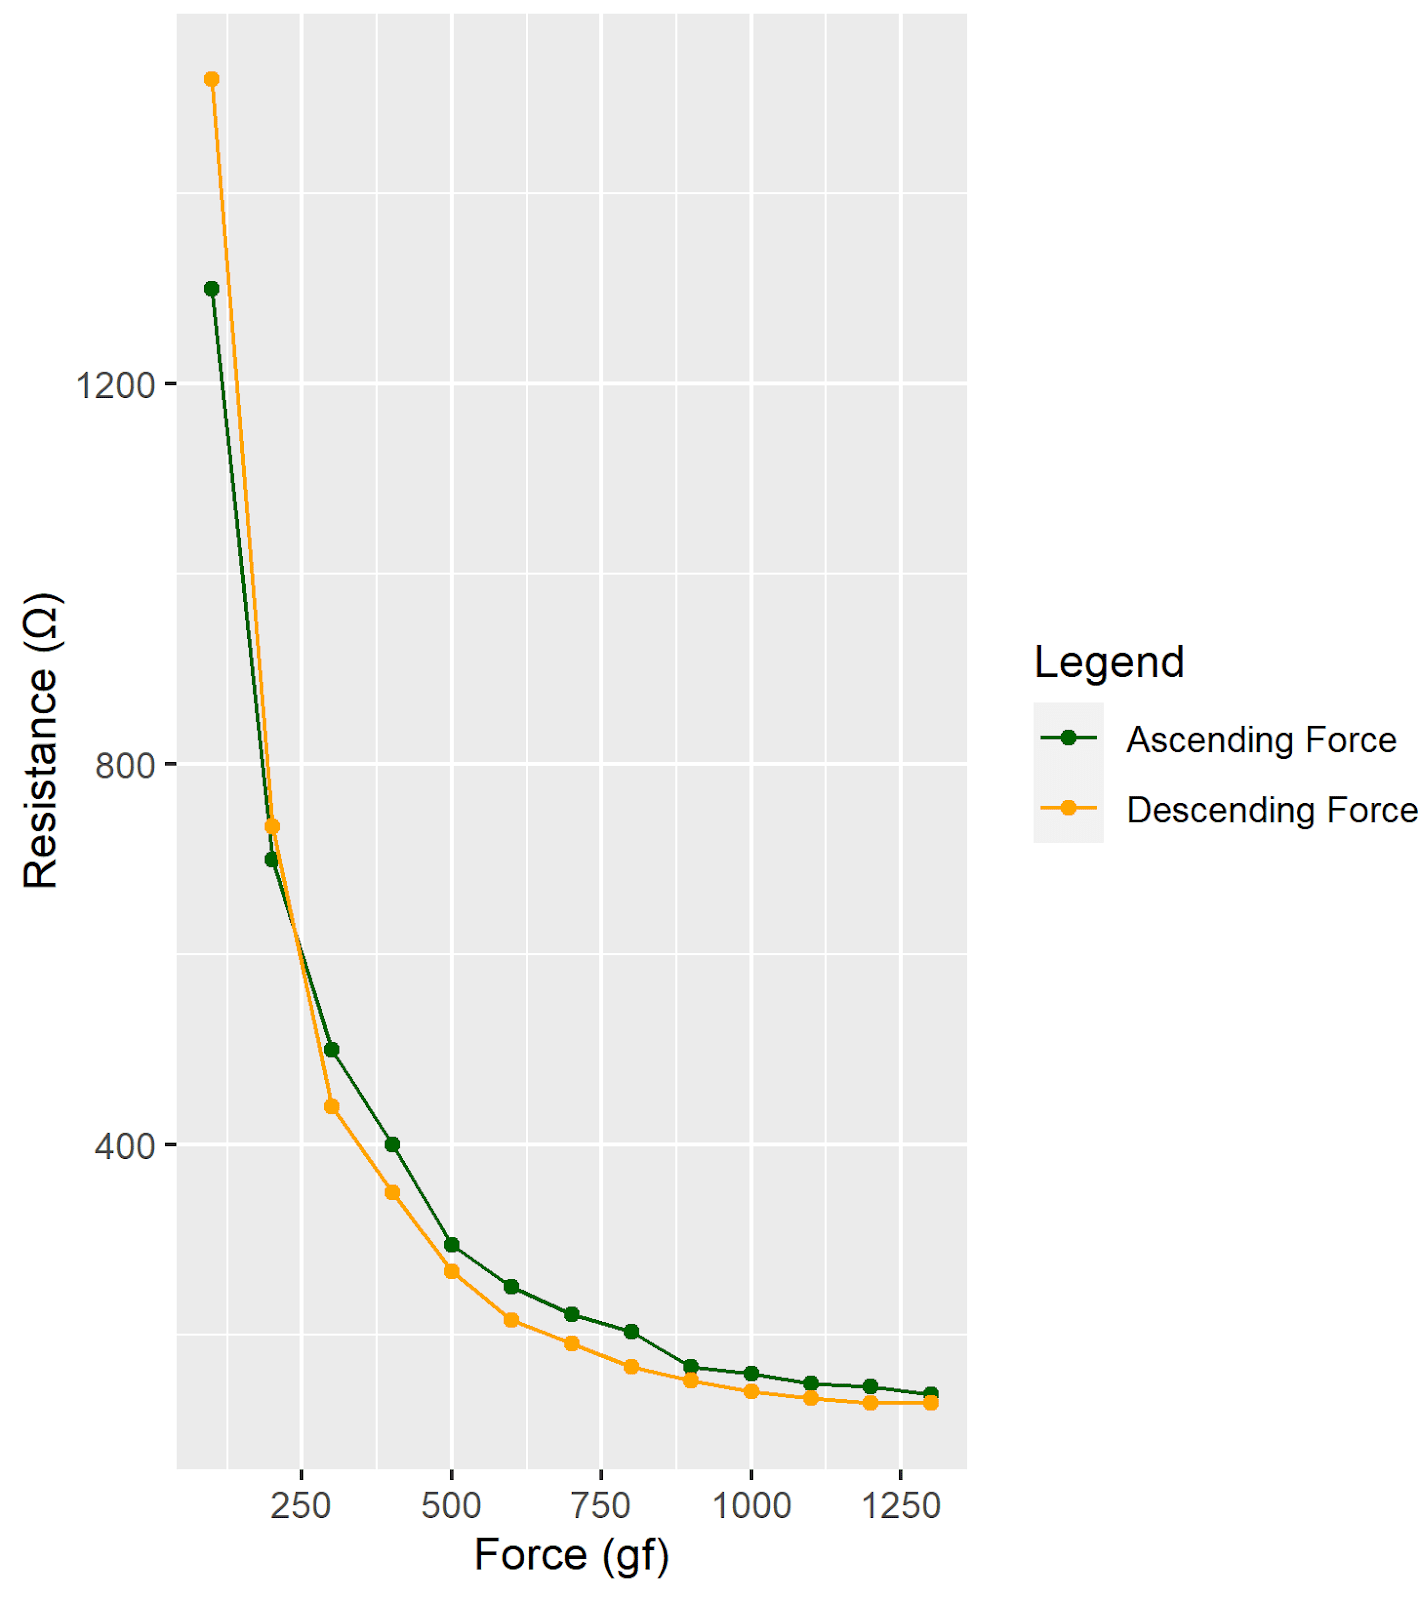
\includegraphics[width=0.5\textwidth]{figs/ascending_descending.png}
      \vspace{-0.2cm}
      \caption[Resistance vs Pressure Relationship]{Resistance vs Pressure Relationship for Velostat}
      \label{fig:velostat}
\vspace{1.0cm}
\end{figure} Comparing the curves under ascending and descending forces it can be seen that hysteresis effects are tolerable. Comparing two layers of Velostat against one layer, it was revealed that the time for a stable result was longer in the case of two layers, although the sensitivity improved in the former case. Therefore one layer of Velostat is appropriate for the pressure mats. \begin{figure}
    \centering
    \begin{subfigure}[b]{0.4\textwidth}
        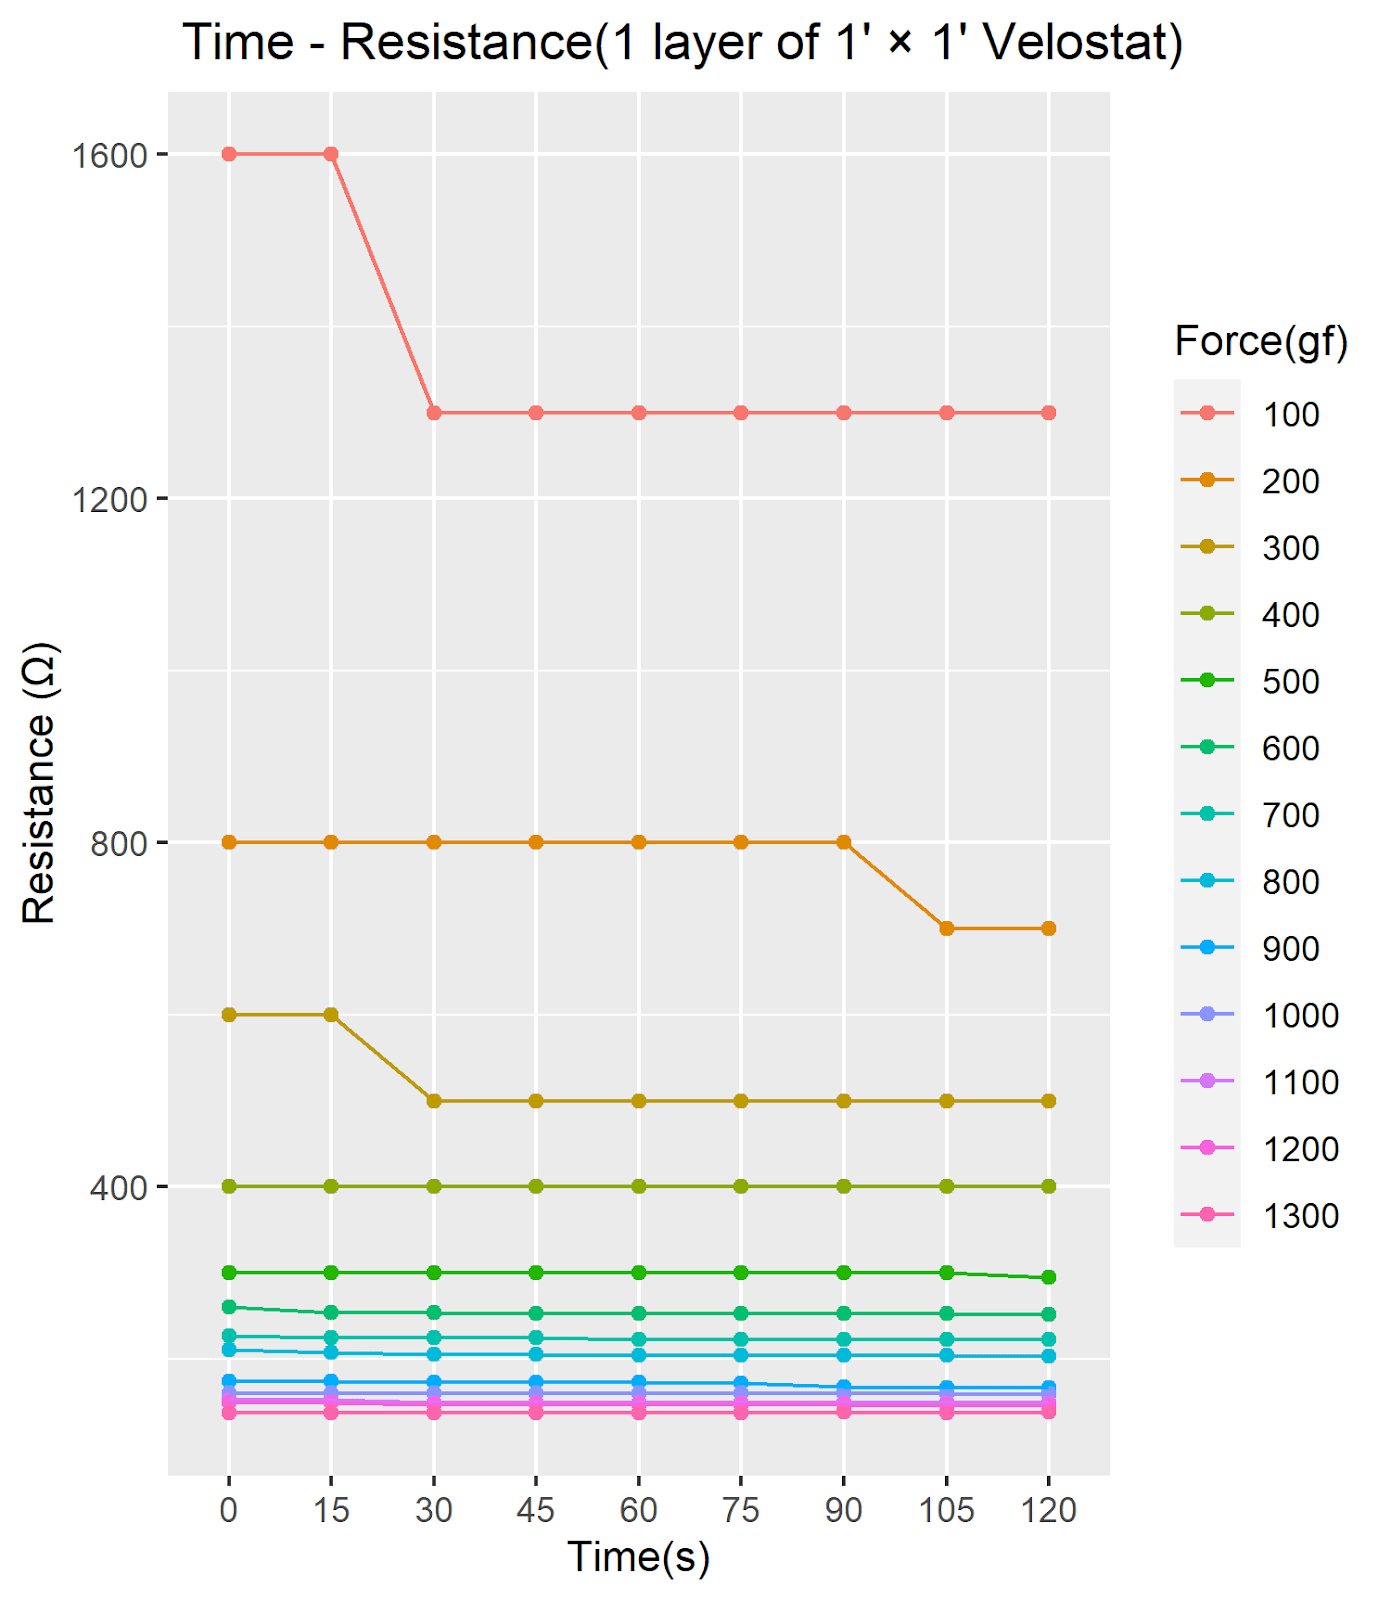
\includegraphics[width=\textwidth]{figs/one_layer.png}
        \caption{One layer of Velostat}
        \label{fig:one_layer}
    \end{subfigure}
    ~ %add desired spacing between images, e. g. ~, \quad, \qquad, \hfill etc. 
      %(or a blank line to force the subfigure onto a new line)
    \begin{subfigure}[b]{0.4\textwidth}
        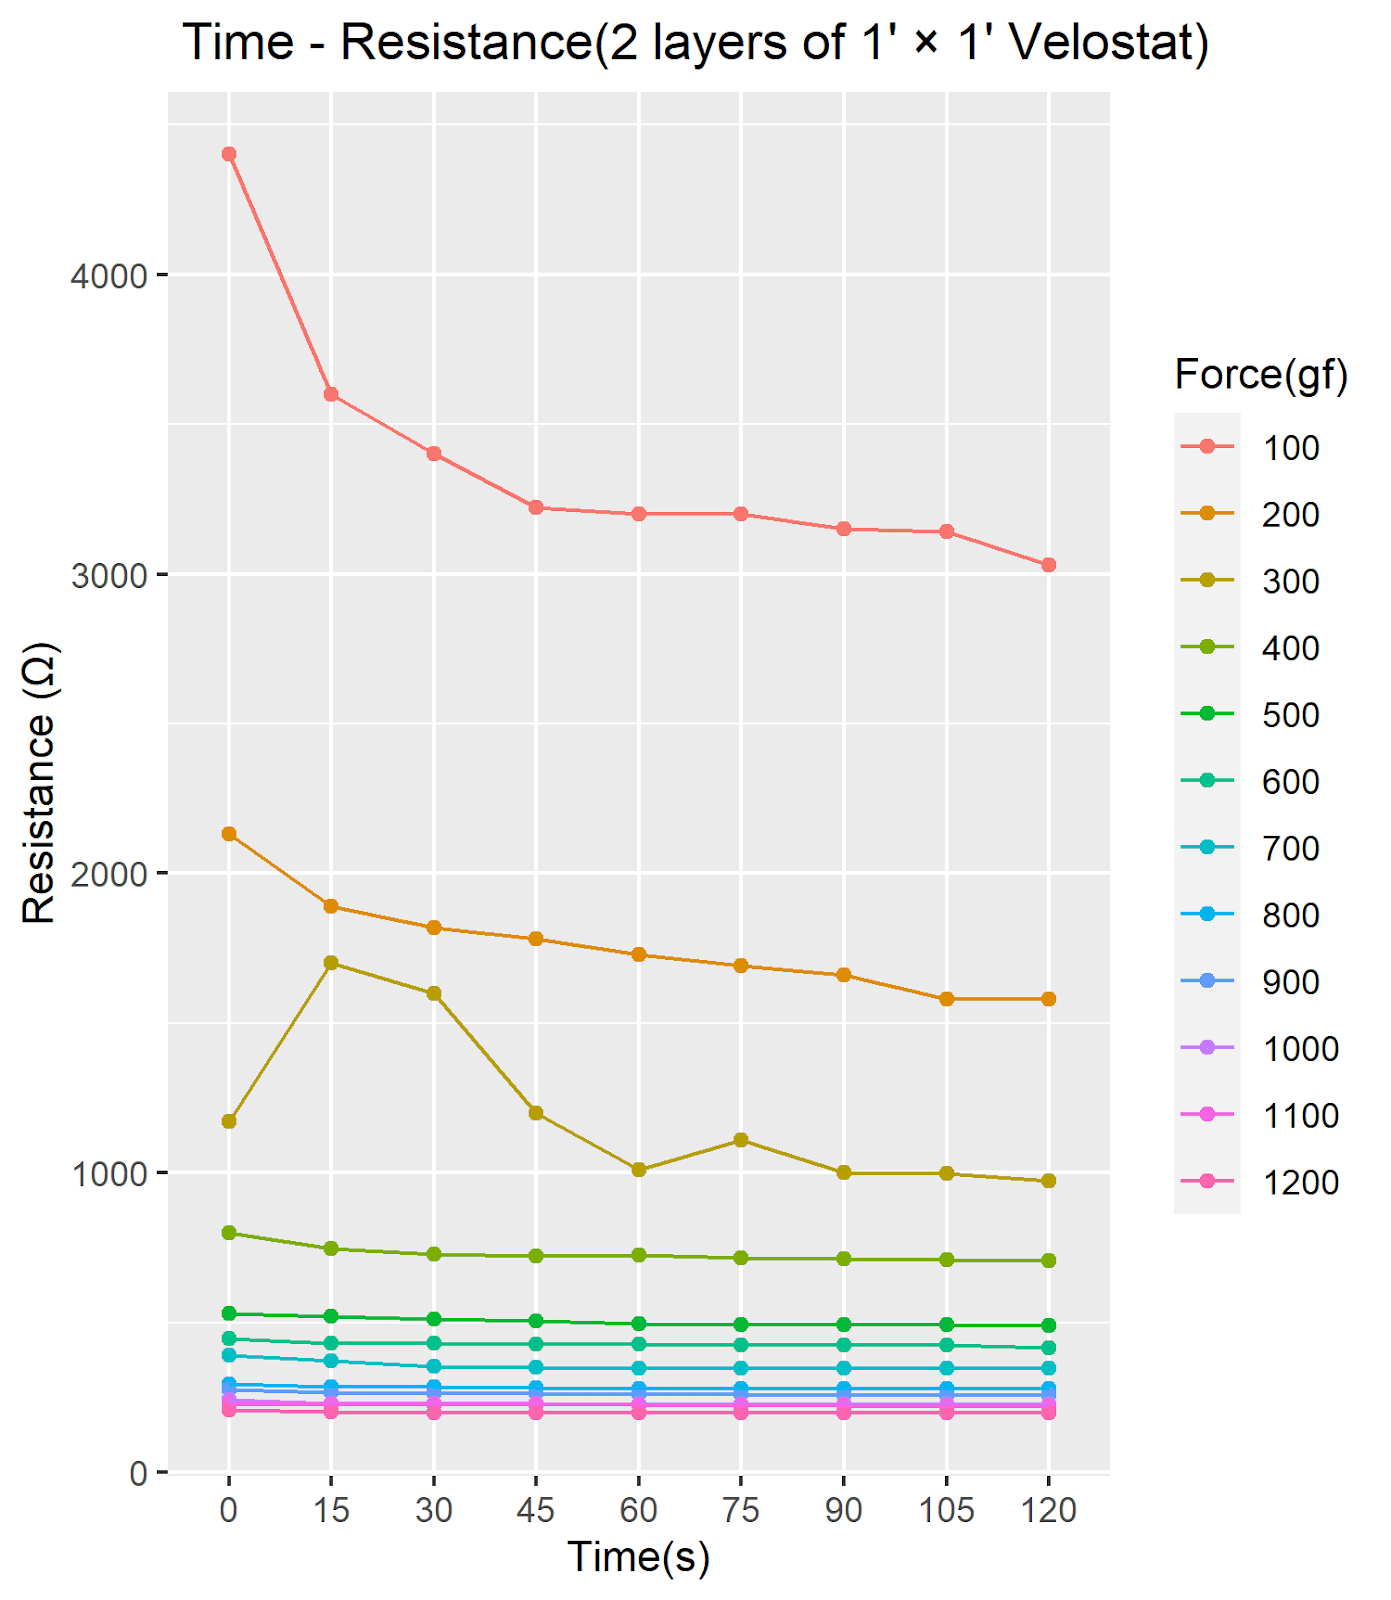
\includegraphics[width=\textwidth]{figs/two_layer.png}
        \caption{Two layers of Velostat}
        \label{fig:two_layer}
    \end{subfigure}
    \hfill %add desired spacing between images, e. g. ~, \quad, \qquad, \hfill etc. 
    %(or a blank line to force the subfigure onto a new line)
    \vspace{0.2cm}
    \caption[Compare No. of Layers]{Time for stable resistance value was higher in the case of two layers than one layer}\label{fig:hysterisis}
\end{figure}


\section{Frames of Pressure Mat Readings}
The frames from the pressure mat are mapped with the colour scheme Jet and Gaussian interpolation is used to get the final output. Since there were huge difficulties for a proper and careful calibration in the overall pressure mat we could not get highly satisfactory results. But the mat detected areas corresponding to high pressure approximately. A more satisfactory image was obtained for feet when standing on the mattress. Disks each weighs 1.25 kg were used to calibrate parts of the mattress. \begin{figure*}
    \vspace{-0.7cm}
      \centering
      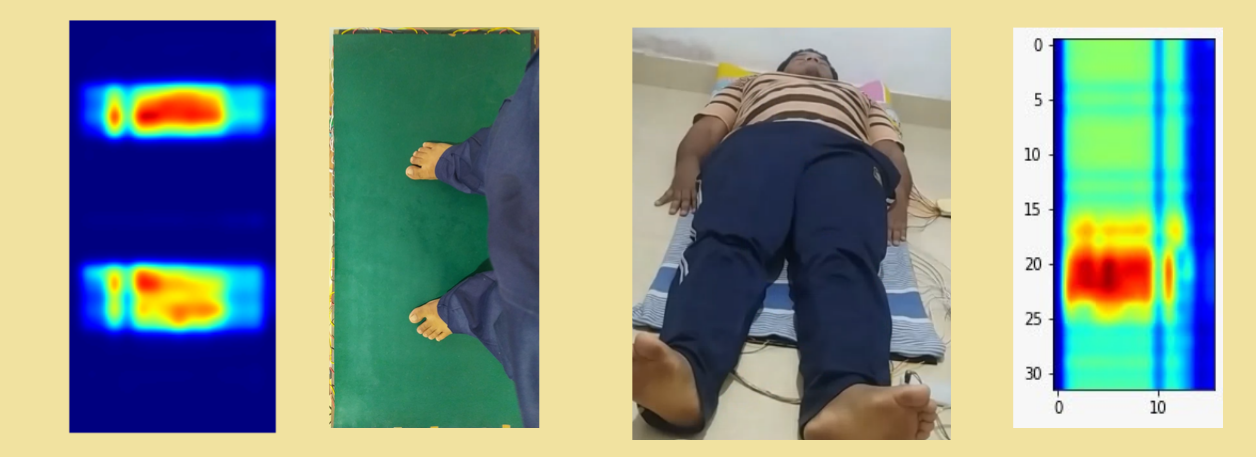
\includegraphics[width=\textwidth]{figs/mat_frames.png}
      \vspace{-0.2cm}
      \caption[Mat frames]{Pressure mat frames}
      \label{fig:mat_frames}
\vspace{1.0cm}
\end{figure*}

\section{Neural Network results}
When a pressure image is sent to the server, the posture detection model detects the posture. Then particular ulceration points are active for that posture. Providing the pressure image and naming these ulceration points as the input, bounding box parameters can be obtained.
All five postures are classified correctly, and bounding boxes are marked appropriately as in the figures.\begin{figure*}[t]
    \vspace{-0.7cm}
      \centering
      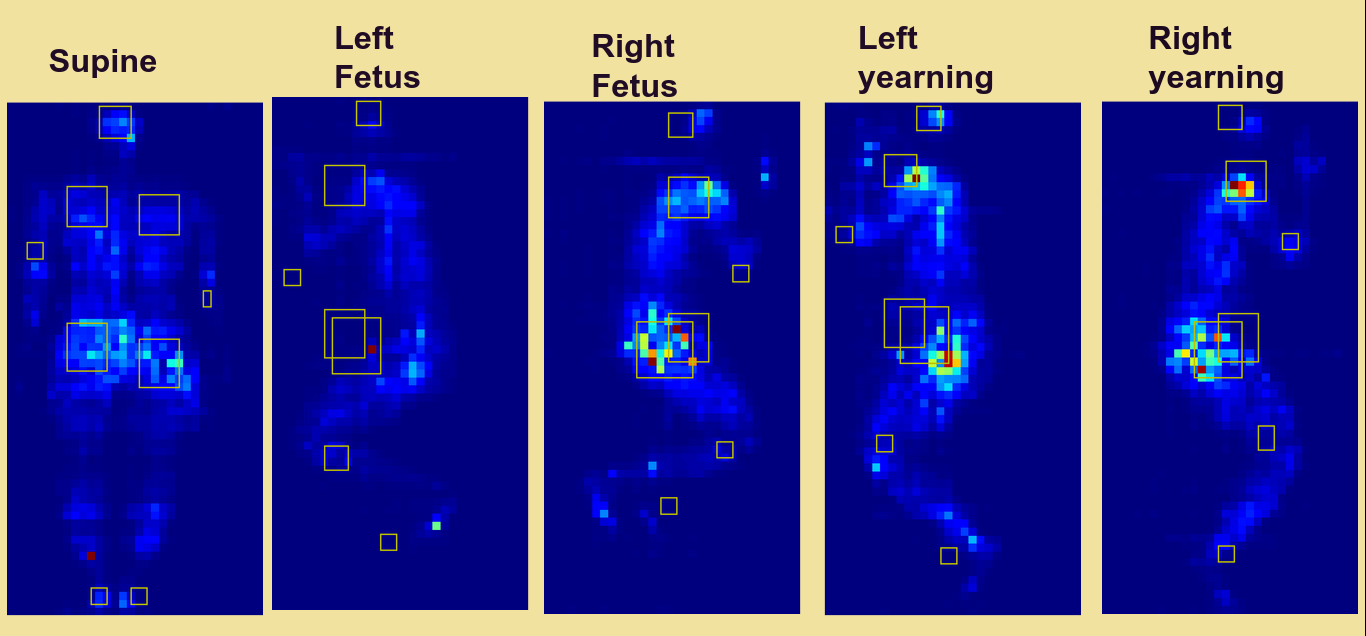
\includegraphics[width=\textwidth]{figs/ml_result.png}
      \vspace{-0.2cm}
      \caption[Results from Neural Network Models]{Results from Neural Network Models}
      \label{fig:mlresult}
\vspace{1.0cm}
\end{figure*}

\section{Simulation of pressure-time behaviour on ulceration points}

When ulceration points are located, the pressure of these points can be calculated. We simulated temporal behaviour and repositioning using the dataset by the University of Dallas. Repositioning considerably shifts the pressure distribution and the pressure values are almost stable in a particular posture.

\begin{figure*}
    \vspace{-0.7cm}
      \centering
      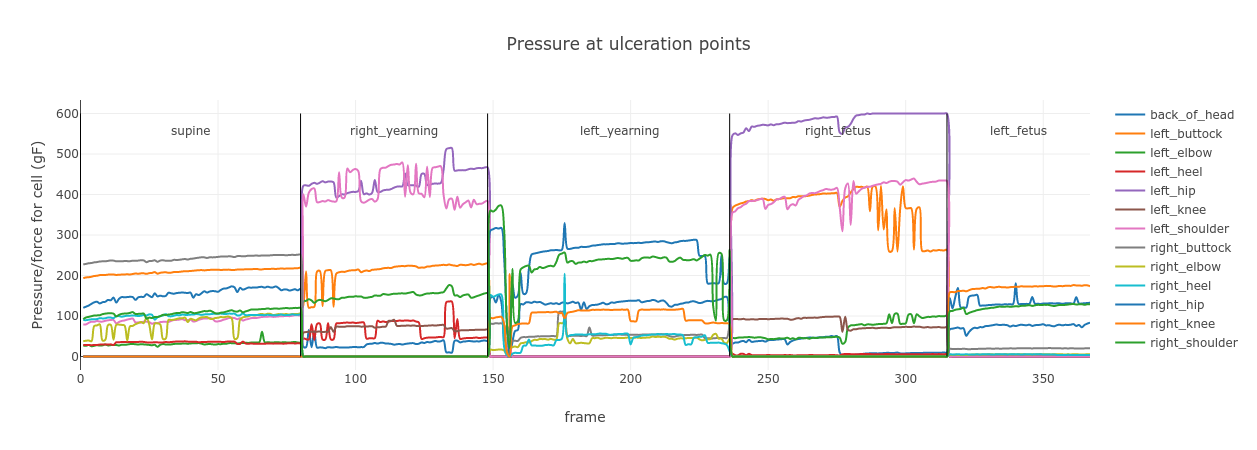
\includegraphics[width=\textwidth]{figs/simulation.png}
      \vspace{-0.2cm}
      \caption[Simulation]{Simulation.}
      \label{fig:simulation}
\vspace{1.0cm}
\end{figure*}

\section{Implementation}

\begin{description}
    \item[The information system]   \url{http://prevelcer.herokuapp.com}
    \item[App] React native based app
    \item[API documentation] \url{https://documenter.getpostman.com/view/13647586/TVmHDeox}
    \item[Neural Network Models] \url{http://prevelcernn.herokuapp.com}
\end{description}




